\setlength{\parskip}{\baselineskip}
\section{Results}

\begin{frame}
	\huge Results
\end{frame}

\begin{frame}
	FPGA Implementation Analysis

    Comparison with Other Technologies
    
    FL \& FPGA Interaction Analysis \& Comparison
\end{frame}



\begin{frame}{FPGA Implementation Analysis - Timing Analysis}
	\begin{minipage}{0.25\textwidth}
    	\begin{figure}[H]
            \centering
    		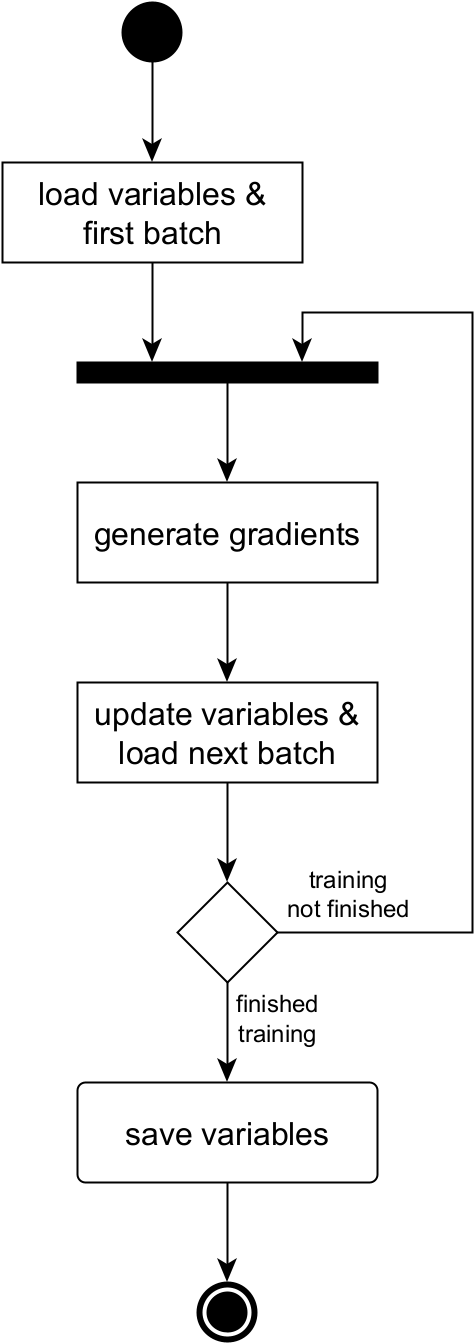
\includegraphics[height=0.8\textheight]{Images/Diagrams/accel_top.png}
    	\end{figure}%
	\end{minipage}%
	\begin{minipage}{0.75\textwidth}
	Latency of training for a single epoch:
        \begin{equation*}
            \small
            Accel_{latency} = I + e \cdot \frac{d}{b} [ G(b) + U ] + S
        \end{equation*}
        Where:
        \begin{table}[H]
            \center
            \small
            \begin{tabular}
                { l @{ $=$ } l | l @{ $=$ } l }
                $I$ & Initialize arrays & $G$ & Generate gradients\\
                $U$ & update variables  & $S$ & Save variables\\
                \multicolumn{4}{c}{}\\
                $e$ & local epochs & $d$ & dataset size\\
                $b$ & batch size\\
            \end{tabular}
        \end{table}
	\end{minipage}%
\end{frame}

\begin{frame}{FPGA Implementation Analysis - Timing Analysis}
    \begin{minipage}{0.3\textwidth}
        G(b) transforms to:
    \end{minipage}%
    \begin{minipage}{0.4\textwidth}
        \center
        $G(b) = G_{up} + b \cdot E + G_{down}$
    \end{minipage}%
    
    \begin{minipage}{0.25\textwidth}
        Where:
    \end{minipage}%
    \begin{minipage}{0.5\textwidth}
        \begin{table}[H]
            \center
            \small
            \begin{tabular}
                { l @{ $=$ } l }
                $G_{up}$ & latency to wind-up the pipeline\\
                $G_{down}$ & latency to wind-down the pipeline\\
                $E$ & latency added by one example\\
            \end{tabular}
        \end{table}
    \end{minipage}%
    
    For a single epoch with the whole dataset (e = 1 \& d = 60000):
    \begin{equation*}
        Accel_{latency} = I + S + 60000 [ E + \frac{ G_{up} + G_{down} + U }{b} ]
    \end{equation*}
    If small batches are important, $U$ is an easy target for optimization.
\end{frame}

\begin{frame}{FPGA Implementation Analysis - Timing Analysis}
    \begin{minipage}{0.3\textwidth}
        Final latency:
    \end{minipage}%
    \begin{minipage}{0.4\textwidth}
        \center
        $Accel_{latency} = 8.157 + \frac{ 14.794 }{b} (sec)$ % 1999224613 + 3625860000/b 
    \end{minipage}%
    
    Due to a bug in Vitis HLS 2022.1, full accuracy facc, fmacc, etc. are unavailable. Instead fadd is used and the clock is restricted at 245MHz. With accumulators the clock can easily be raised to 300 MHz.
    
    \begin{minipage}{0.3\textwidth}
        With accumulators:
    \end{minipage}%
    \begin{minipage}{0.4\textwidth}
        \center
        $Accel_{latency} = 6.664 + \frac{ 12.086 }{b} (sec)$ % 1999224613 + 3625860000/b
    \end{minipage}%
\end{frame}

\begin{frame}{FPGA Implementation Analysis - Timing Analysis}
    \begin{minipage}{0.5\textwidth}
        \begin{figure}[H]
            \center
            \begin{tikzpicture}
                \begin{axis}[
                    xmode = log,
                    log ticks with fixed point,
                    ymin = 0,
                    ymax = 30,
                    xmin = 1,
                    xmax = 60000,
                    ylabel = Latency (sec),
                    xlabel = Batch size,
                    width = \textwidth,
                    label style = { font=\footnotesize },
                    tick label style = { font=\footnotesize } 
                ]
                    \addplot[ domain = 1:60000, color = blue ] { 8.156836421 + 14.793508800 / x };
                    \addplot[ domain = 1:60000, color = red ] { 6.664082036 + 12.086199879 / x };
                    \addlegendentry{\footnotesize$Accel$}
                    \addlegendentry{\footnotesize$Accel\:with\:facc$}
                \end{axis}
            \end{tikzpicture}
        \end{figure}
    \end{minipage}%
    \begin{minipage}{0.5\textwidth}
        \begin{itemize}
            \item For batch size $\sim$50 or more, the second part of the equation is insignificant
            \item Average consumption of 9.356 W
        \end{itemize}
    \end{minipage}%
\end{frame}

% \begin{frame}{FPGA Implementation Analysis - Power Consumption Analysis}
%     \begin{minipage}{0.5\textwidth}
%     	\begin{figure}[H]
%             \centering
%     		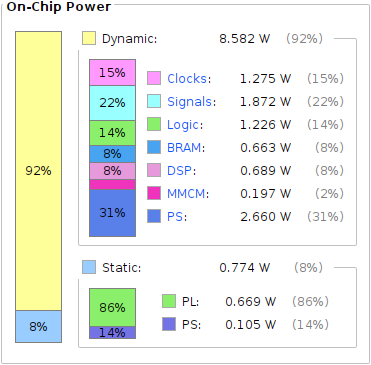
\includegraphics[width=0.8\textwidth]{Images/Diagrams/power.png}
%     	\end{figure}%
%     \end{minipage}%
%     \begin{minipage}{0.5\textwidth}
%         \begin{itemize}
%             \item average consumption of 9.356 W
%             \item Post place and route estimation
%             \item CPU mostly sleeps in blocking calls, no major power consumption
%         \end{itemize}
%     \end{minipage}%
% \end{frame}

\begin{frame}{Comparison with other technologies - Specifications of Compared Platforms - i7-9750H}
    CPU: i7-9750H\\
    \begin{itemize}
        \item released in 2019
        \item aimed for mobile platforms (laptops, tablets, etc.).
    \end{itemize}
    \begin{table}[H]
        \center
        \begin{tabular}
            { l | l }
            Core / Threads & 6 / 12\\
            Clock Frequency & 2.6 - 4.5 GHz\\
            Cache & 12 MB Intel Smart Cache\\
            Supplied Memory & 16GB DDR4-2666\\
            Max Memory Bandwidth & 41.8 GB/s $\times$ 2 channels\\
            Instruction Set Extensions & SSE4.1, SSE4.2, AVX2\\
            Average Power Consumption & 45 W\\
        \end{tabular}
        % \caption{i7-9750H specifications}
    \end{table}
\end{frame}

\begin{frame}{Comparison with other technologies - Specifications of Compared Platforms - GTX1660Ti}
    GPU: GTX1660Ti\\
    \begin{itemize}
        \item released in 2019
        \item aimed for mobile platforms (laptops, tablets, etc.).
    \end{itemize}
    \begin{table}[H]
        \center
        % \small
        \begin{tabular}
            { l | l }
            CUDA cores & 1536\\
            Clock Speed & 1500 - 1770 MHz\\
            Memory Configuration & 6GB GDDR6, 1500 MHz\\
            Memory Interface & 192-bit\\
            Memory Bandwidth & 288 GB/s\\
            Single Precision Compute Power & 5437.44 GFLOPS\\
            % Compute Capability & 7.5\\
            Average Power Consumption & 120 W\\
        \end{tabular}
        % \caption{GTX 1660 Ti specifications}
    \end{table}
\end{frame}

\begin{frame}{Comparison with other technologies - Latency}

    \begin{minipage}{0.5\textwidth}
        \begin{figure}[H]
            \center
            \begin{tikzpicture}
                \begin{axis}[
                    xmode = log,
                    log ticks with fixed point,
                    ymin = 0,
                    ymax = 110,
                    xmin = 1,
                    xmax = 60000,
                    ylabel = Latency (sec),
                    xlabel = Batch size,
                    width = \textwidth,
                    no markers,
                    label style = { font=\footnotesize },
                    tick label style = { font=\footnotesize } 
                ]
                    \addplot[ domain = 1:60000 , color = blue ] { 8.166836421 + 14.793508800 / x };
                    \addlegendentry {\footnotesize$FPGA$}
                    
                    \addplot+ [ forget plot , name path=upper_gpu , draw=none ] table[ smooth , tension=.8 , x=batch_size , y=latency_max ] {data/gpu_latency_per_batch_size.dat};
                    \addplot [ name path=lower_gpu , color=red ] table[ smooth , tension=.8 , x=batch_size , y=latency_min ] {data/gpu_latency_per_batch_size.dat};
                    \addplot+ [ forget plot , fill=red!25 ] fill between[ of=upper_gpu and lower_gpu ];
                    \addlegendentry {\footnotesize$GPU$}
        
                    \addplot+ [ name path=upper_cpu , color=green ] table[ smooth , tension=.8 , x=batch_size , y expr = ( \thisrow{latency_max} + \thisrow{latency_min} ) / 2 ] {data/cpu_latency_per_batch_size.dat};
                    \addlegendentry {\footnotesize$CPU$}
                
                \end{axis}
            \end{tikzpicture}
        \end{figure}
    \end{minipage}%
    \begin{minipage}{0.5\textwidth}
        \hspace{0.35cm}Train a single epoch with the whole\newline\hspace*{0.35cm}dataset (60000 samples).
        \begin{itemize}
            \item FPGA faster for small batches
            \item overtaken by GPU over large batches
            \item GPU shows great variance
            \item CPU consistently slower than the other options
            % \item GPU can not run non-stochastic gradient descent. Not enough GPU memory for huge batches.
        \end{itemize}
    \end{minipage}%
\end{frame}

% \begin{frame}{Comparison with other technologies - Power Consumption}
%     Due to clock frequency boosting, the CPU has greater power consumption than the listed value. 
    
%     \begin{table}[H]
%         \center
%         \begin{tabular}
%             { | c | c | c | }
%             \hline
%             CPU & GPU & FPGA\\
%             \hline
%             53 W & 120 W & 9.356 W\\ 
%             \hline
%         \end{tabular}
%         \caption*{Power consumption of the three implementations.}
%     \end{table}
    
%     The FPGA consumes:\\
%     \begin{itemize}
%         \item 5.67× less power than the CPU
%         \item 12.83× less power than the GPU
%     \end{itemize}
% \end{frame}

\begin{frame}{FL \& FPGA Interaction Analysis \& Comparison - Methodology}
    Throughput comparison is inadequate!
    \begin{equation*}
        FL_{latency} = GE_{num} \times GE_{latency}
    \end{equation*}
    
    As shown in Robustness Analysis, the number of GEs depends on multiple factors. 

    The following experiments focus on the most important one, the batch size. 
    
    Repeated with different LR decay values. Only best results are shown.
\end{frame}

\begin{frame}{FL \& FPGA Interaction Analysis \& Comparison - Methodology}
    Only a single FPGA/GPU available. Real-time FL is impossible. Instead:\\
    \begin{itemize}
        \item Train on CPU to find the number GEs required to reach target accuracy.
        \item Replace the training latency with that of the desired device.
    \end{itemize}
    
    Communication latency can be approximated:\\
    \begin{itemize}
        \item $\frac{ Message\_size_{bits} }{ Communication\_speed_{bps} }$
        \item Server communication speed: 1Gbps Up, 1Gbps Down.
        \item Client communication speed: 10Mbps Up, 1Mbps Down.
    \end{itemize}
\end{frame}

\begin{frame}{FL \& FPGA Interaction Analysis \& Comparison - IID dataset - Setting}
    The Fashion-MNIST dataset is split randomly and evenly across 10 clients. Federated Averaging is used.
    \begin{table}[H]
        \center
        \begin{tabular}
            { | l | c | }
            \hline
            parameters & FedAvg\\\hline
            total clients   & 10\\\hline
            clients per GE  & 5\\\hline
            local epochs    & 1\\\hline
            initial LR      & 1e-2\\\hline
        \end{tabular}
        \caption*{Parameters of the IID FL experiment.}
    \end{table}
    Target accuracy is set at 91\%.
\end{frame}

\begin{frame}{FL \& FPGA Interaction Analysis \& Comparison - IID dataset - Convergence}
    \begin{minipage}{0.5\textwidth}
        \begin{figure}[H]
            \center
            \begin{tikzpicture}
                \begin{axis}[
                    ybar,
                    bar width = 6pt,
                    ylabel = Global Epochs,
                    ymin = 0,
                    ymax = 200,
                    xlabel = Batch size,
                    symbolic x coords = {5,6,8,10,12,15,16,20,24,25,30,40,48,50,60,75,100,120,125,150,200},
                    xtick style = {draw=none},
                    enlarge x limits={abs=5pt},
                    width = \textwidth,
                    height = 0.8\textheight,
                    label style = { font=\footnotesize },
                    tick label style = { font=\footnotesize }
                ]
                    \addplot [ black , fill = blue!50 ] table [ x = batch_size , y = global_epochs] {data/IID_epochs.dat};
                \end{axis}
            \end{tikzpicture}
            \caption*{GEs to reach 91\% accuracy, per batch size.}
        \end{figure}
    \end{minipage}%
    \begin{minipage}{0.5\textwidth}
        \begin{itemize}
            \item Batch sizes 8 \& 10 require the least GEs, 28.
            \item for batch sizes smaller than 5 or larger than 200, the model does not converge or require over 200 GEs.
        \end{itemize}
    \end{minipage}
\end{frame}

\begin{frame}{FL \& FPGA Interaction Analysis \& Comparison - IID dataset - Total time}
    \begin{figure}[H]
        \centering
        \addtolength{\leftskip} {-2cm} % increase (absolute) value if needed
        \addtolength{\rightskip}{-2cm}
        
        \begin{tikzpicture} [
            /pgfplots/every axis/.style = {
                ybar stacked ,
                bar width = 7pt,
                ymin = 0 ,
                ymax = 1000 ,
                ytick distance = 250 ,
                ylabel = Global Training time (sec) ,
                symbolic x coords = {5,6,8,10,12,15,16,20,24,25,30,40,48,50,60,75,100,120,125,150,200} ,
                enlarge x limits = 0.03 ,
                xtick = data,
                xtick style = { draw = none } ,
                xlabel = Batch size,
                width = 1 \textwidth ,
                height = 0.85 \textheight ,
                label style = { font=\footnotesize },
                tick label style = { font=\footnotesize }
            }
        ]
            \begin{axis}[ bar shift = -3.5pt , ]
                \addplot [ black , fill = blue!75 ] 
                    table [ 
                        y expr = { \thisrow{global_epochs} * ( 0.82568 + 1.47935 / \thisrow{batch_size} ) } , 
                        x = batch_size ,
                        meta expr = { \thisrow{global_epochs} * ( 0.82568 + 1.47935 / \thisrow{batch_size} ) } 
                    ] {data/IID_epochs.dat};  % training cost
    
                \addplot [ black , fill = blue!25 ,
                    point meta = y ,
                    nodes near coords = \pgfmathprintnumber\pgfplotspointmeta ,
                    every node near coord/.append style = {
                        font=\footnotesize ,
                        anchor = west ,
                        rotate = 90 ,
                        yshift = 4pt ,
                        /pgf/number format/.cd , precision = 0 ,
                    }
                ] 
                    table [ 
                        y expr = { \thisrow{global_epochs} * 3.73 } , 
                        x = batch_size , 
                        meta expr = { \thisrow{global_epochs} * 3.73 } ,
                    ] {data/IID_epochs.dat}; % communication cost 
                    \label{FPGA_iid} 
            \end{axis}
            
            \begin{axis}[ hide axis , bar shift = 3.5pt , legend pos = north west , ]
                \addplot [ forget plot , black , fill = red!75 ] 
                    table [ 
                        y expr = { \thisrow{global_epochs} * ( \thisrow{gpu_lat_per_epoch} ) } , 
                        x = batch_size ,
                        meta expr = { \thisrow{global_epochs} * ( \thisrow{gpu_lat_per_epoch} ) } 
                    ] {data/IID_epochs.dat};  % training cost
    
                \addplot [ black , fill = red!25 , 
                    point meta = y ,
                    nodes near coords = \pgfmathprintnumber\pgfplotspointmeta ,
                    every node near coord/.append style = {
                        font=\footnotesize ,
                        anchor = west ,
                        rotate = 90 ,
                        yshift = -4pt ,
                        /pgf/number format/.cd , precision = 0
                    }
                ]
                    table [
                        y expr = { \thisrow{global_epochs} * 3.73 } ,
                        x = batch_size ,
                        meta expr = { \thisrow{global_epochs} * 3.73 }
                    ] {data/IID_epochs.dat}; % communication cost
    
                \addlegendentry{\footnotesize GPU}
                \addlegendimage{ /pgfplots/refstyle=FPGA_iid }\addlegendentry{\footnotesize FPGA}
            \end{axis}
        \end{tikzpicture}
    \end{figure}
\end{frame}

\begin{frame}{FL \& FPGA Interaction Analysis \& Comparison - Non-IID dataset - Setting}
    The Fashion-MNIST dataset is split between 5 clients. Each client is the exclusive owner of two labels. Federated Averaging is used.
    \begin{table}[H]
        \center
        \begin{tabular}
            { | l | c | }
            \hline
            parameters & FedAvg\\\hline
            total clients   & 5\\\hline
            clients per GE  & 5\\\hline
            local epochs    & 1\\\hline
            initial LR      & 1e-2\\\hline
        \end{tabular}
        \caption*{Parameters of the non-IID FL experiment.}
    \end{table}
    Target accuracy is set at 85\%.
\end{frame}

\begin{frame}{FL \& FPGA Interaction Analysis \& Comparison - Non-IID dataset - Convergence}
    \begin{minipage}{0.5\textwidth}
        \begin{figure}[H]
            \center
            \begin{tikzpicture}
                \begin{axis}[
                    ybar,
                    ylabel = Global Epochs,
                    xlabel = Batch size,
                    xtick = data,
                    symbolic x coords = {4,5,6,8,10,12,15,16,24},
                    xtick style = {draw=none},
                    nodes near coords,
                    every node near coord/.append style = {
                        font=\footnotesize ,
                        /pgf/number format/.cd , precision = 0 ,
                    },
                    width = \textwidth,
                    height = 0.8\textheight,
                    label style = { font=\footnotesize },
                    tick label style = { font=\footnotesize }
                ]
                    \addplot [ black , fill = blue!50 ] table [ x = batch_size , y = global_epochs] {data/nonIID_epochs.dat};
                \end{axis}
            \end{tikzpicture}
            \caption*{GEs to reach 85\% accuracy, per batch size.}
        \end{figure}  
    \end{minipage}%
    \begin{minipage}{0.5\textwidth}
        \begin{itemize}
            \item Few batch sizes reach the target accuracy.
        \end{itemize}
    \end{minipage}
\end{frame}


\begin{frame}{FL \& FPGA Interaction Analysis \& Comparison - Non-IID dataset - Total time}
    \begin{figure}[H]
        \center
        \begin{tikzpicture} [
            /pgfplots/every axis/.style = {
                ylabel = Global Training time (sec) ,
                ybar stacked ,
                ymin = 0 ,
                ymax = 2250 ,
                ytick distance = 500 ,
                symbolic x coords = {4,5,6,8,10,12,15,16,24} ,
                xlabel = Batch size ,
                xtick = data ,
                xtick style = { draw = none } ,
                enlarge x limits = 0.075 ,
                bar width = 10pt ,
                width = 0.8 \textwidth ,
                height = 0.85 \textheight ,
                label style = { font=\footnotesize },
                tick label style = { font=\footnotesize }
            },
        ]
            \begin{axis}[ bar shift = -5pt , ]
                \addplot [ black , fill = blue!75 ] 
                    table [ 
                        y expr = { \thisrow{global_epochs} * ( 1.641 + 2.9587 / \thisrow{batch_size} ) } , 
                        x = batch_size ,
                        meta expr = { \thisrow{global_epochs} * ( 1.641 + 2.9587 / \thisrow{batch_size} ) } 
                    ] {data/nonIID_epochs.dat};  % training cost
    
                \addplot [ black , fill = blue!25 ,
                    point meta = y ,
                    nodes near coords = \pgfmathprintnumber\pgfplotspointmeta ,
                    every node near coord/.append style = {
                        anchor = west ,
                        rotate = 90 ,
                        yshift = 5pt ,
                        /pgf/number format/.cd , precision = 0 ,
                    },
                ] 
                    table [ 
                        y expr = { \thisrow{global_epochs} * 3.73 } , 
                        x = batch_size , 
                        meta expr = { \thisrow{global_epochs} * 3.73 } ,
                    ] {data/nonIID_epochs.dat}; % communication cost 
                    \label{FPGA} 
            \end{axis} 
            
            \begin{axis}[ hide axis , bar shift = 5pt , ]
                \addplot [ forget plot , black , fill = red!75 ] 
                    table [ 
                        y expr = { \thisrow{global_epochs} * ( \thisrow{gpu_lat_per_epoch} ) } , 
                        x = batch_size ,
                        meta expr = { \thisrow{global_epochs} * ( \thisrow{gpu_lat_per_epoch} ) } 
                    ] {data/nonIID_epochs.dat};  % training cost
    
                \addplot [ black , fill = red!25 , 
                    point meta = y,
                    nodes near coords = \pgfmathprintnumber\pgfplotspointmeta ,
                    every node near coord/.append style = {
                        anchor = west ,
                        rotate = 90 ,
                        yshift = -5pt ,
                        /pgf/number format/.cd , precision = 0 ,
                    },
                ] 
                    table [ 
                        y expr = { \thisrow{global_epochs} * 3.73 } , 
                        x = batch_size , 
                        meta expr = { \thisrow{global_epochs} * 3.73 } ,
                    ] {data/nonIID_epochs.dat}; % communication cost
                    
                \addlegendentry{\footnotesize GPU}
                \addlegendimage{ /pgfplots/refstyle=FPGA }\addlegendentry{\footnotesize FPGA}
            \end{axis}
        \end{tikzpicture}
    \end{figure}
\end{frame}

\begin{frame}{FL & FPGA Interaction Analysis & Comparison - Summary}
    \begin{minipage}{0.4\textwidth}
        \begin{figure}[H]
            \center
            \begin{tikzpicture}
                \begin{axis}[
                    ylabel = Global Epochs,
                    ymin = 0,
                    ymax = 200,
                    xlabel = Batch size,
                    xmode = log,
                    % scale = 1.25,
                    legend pos = south east ,
                    width = 1.2\textwidth,
                    % height = 0.8\textheight,
                    label style = { font=\footnotesize },
                    tick label style = { font=\footnotesize }
                ]
                    \addplot table [ x = batch_size , y = global_epochs] {data/IID_epochs.dat};
                    \addlegendentry{\footnotesize IID}
                    \addplot table [ x = batch_size , y = global_epochs] {data/nonIID_epochs.dat};
                    \addlegendentry{\footnotesize Non-IID}
                \end{axis}
            \end{tikzpicture}
            % \caption*{GEs to reach target accuracy}
        \end{figure}%
    \end{minipage}%
    \begin{minipage}{0.65\textwidth}

        \begin{table}[H]
            \center
            \small
            \begin{tabular}
                { l c c}
                \hline
                \multirow{2}{*}{ \shortstack{Dataset\\Distribution} } & \multicolumn{2}{c}{Total Time (s)} \\
                             & GPU       & FPGA               \\
                \hline
                IID          & 143       & 132 ($1.08\times$) \\
                non-IID      & 888       & 739 ($1.2\times$)  \\
                \hline
            \end{tabular}
        \end{table}
        \begin{table}[H]
            \center
            \small
            \begin{tabular}
                { l c c }
                \hline
                \multirow{2}{*}{ \shortstack{Dataset\\Distribution} } & \multicolumn{2}{c}{Total Energy (J)}\\
                             & GPU       & FPGA\\
                \hline
                IID          & 4637      & 255 $(18.18\times)$\\ % 38.64 * 120 , 27.26122 * 9.356
                non-IID      & 41.16k     & 2.57k $(16.35\times)$\\ % 343 * 120 , 269 * 9.356
                \hline
            \end{tabular}
        \end{table}
    \end{minipage}
\end{frame}